\section{Solutions on the market}

The following chapter presents the two most popular solutions used in the context of service meshes: Istio and Linkerd. Both technology solutions have in common that they are based on Kubernetes. While Linkerd requires Kubernetes, Istio could also rely on virtual machines. To understand practical solutions of service meshes, it is very helpful to know how Kubernetes works.

\subsection{Kubernetes}

Kubernetes provides a number of functions. It can be seen as a container platform, microservices platform and cloud platform.
It is a common way to use container technologies nowadays. Containers are isolated; they do not have access to processes or file systems of the host or other containers.
Advantages of container solutions are easy creation and deployment of container images that allow continious integration, delivery and test. The role of Kubernetes is to manage and orchestrate these containers \cite{k8s}.

The four main Kubernetes objects are important to understand the role of service meshes in the microservices context:
\begin{itemize}
\item Pods: Pods are the smallest deployable unit that Kubernetes manages. A pod is one or a group of multiple containers that share storage and network resources.
\item Namespaces: Pods can be grouped into what are called namespaces. These represent a kind of virtual cluster. This already represents a kind of security concept. By default, a service from namespace A cannot communicate with a service from namespace B without explicit configuration.
\item Labels: Each Kubernetes deployment can be attached with an arbitrary amount of labels. These labels are simple key/value pairs that allow to group objects in Kubernetes into subsets \cite{k8s}.
\end{itemize}

Service meshes that use Kubernetes extend the functionality by abstracting concepts like automatic sidcar injection. This would be also possible without service meshes, but significantly more complex and less automated.

\subsection{Istio}

As illustrated in figure \ref{fig:arch-istio}, Istio uses a basic control and data plane architecture, as explained in chapter \ref{chap:mesh-architecture}. For the data plane, it uses the sidecar pattern by using \textsc{Envoy} proxies. \textsc{Envoy} a high-performance proxy that already brings features like service discovery, load balancing, circuit breaking and many more \cite{istio-docs-arch}.

\textsc{Istiod} (Istio daemon) provides management for service discovery, configuration and certificates. It converts routing rules into \textsc{Envoy}'s configuration format and also directs the traffic to the sidecar proxies \cite{istio-docs-arch}.

\begin{figure}
    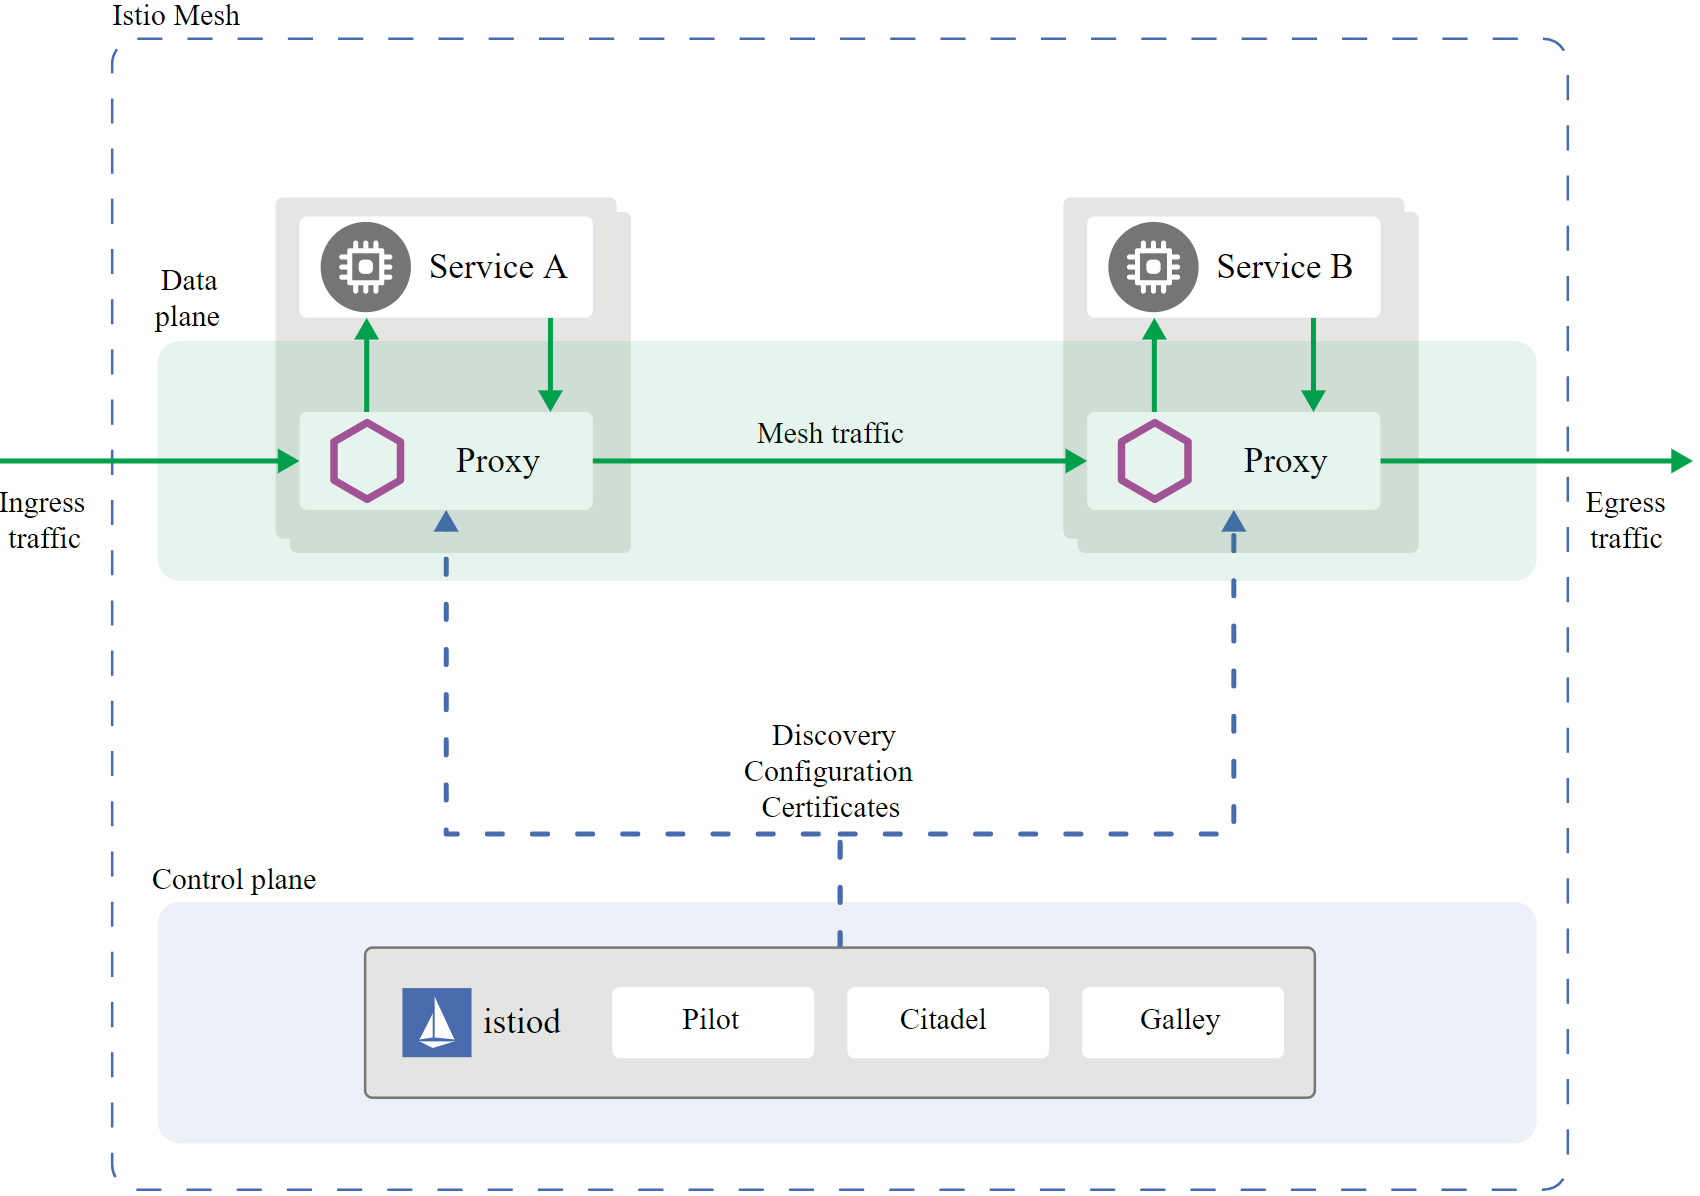
\includegraphics[width=\columnwidth]{img/istio_architecture.png}
    \caption{Architecture of Istio \cite{istio-docs-arch}}
    \label{fig:arch-istio}
\end{figure}

\subsection{Linkerd}

According to Linkerd's documentation \cite{linkerd-docs-arch}, Linkerd also uses a basic control and data plane architecture, as explained in chapter \ref{chap:mesh-architecture}. It also uses the sidecar pattern, but has implemented an own proxy solution named \textsc{Linkerd2-proxy}. Linkerd developers rate \textsc{Envoy} as too complex \cite{linkerd-docs-no-envoy}, which is why they decided to implement their own solution, which they call a "micro-proxy". 
Unlike Istio, Linkerd does not handle ingress traffic. It works in conjunction of every ingress controller of choice, e.g. \textsc{nginx} \cite{linkerd-docs-faq}.

As illustrated in figure \ref{fig:arch-linkerd}, each \textsc{linkerd-proxy} has access to two components: \textsc{identity} and \textsc{destination}.

\textsc{destination} is a lookup-service, where each proxy is able to check where exactly to send requests. \textsc{identity} provides a certificate authority.

While injecting a sidecar proxy on an application service, a route \textsc{/metrics} at port 4191 is exposed to provide log messages and metrics for \textsc{Prometheus}, which is a central logging and monitoring instance which is often used with Kubernetes \cite{linkerd-docs-arch}.

\begin{figure}
    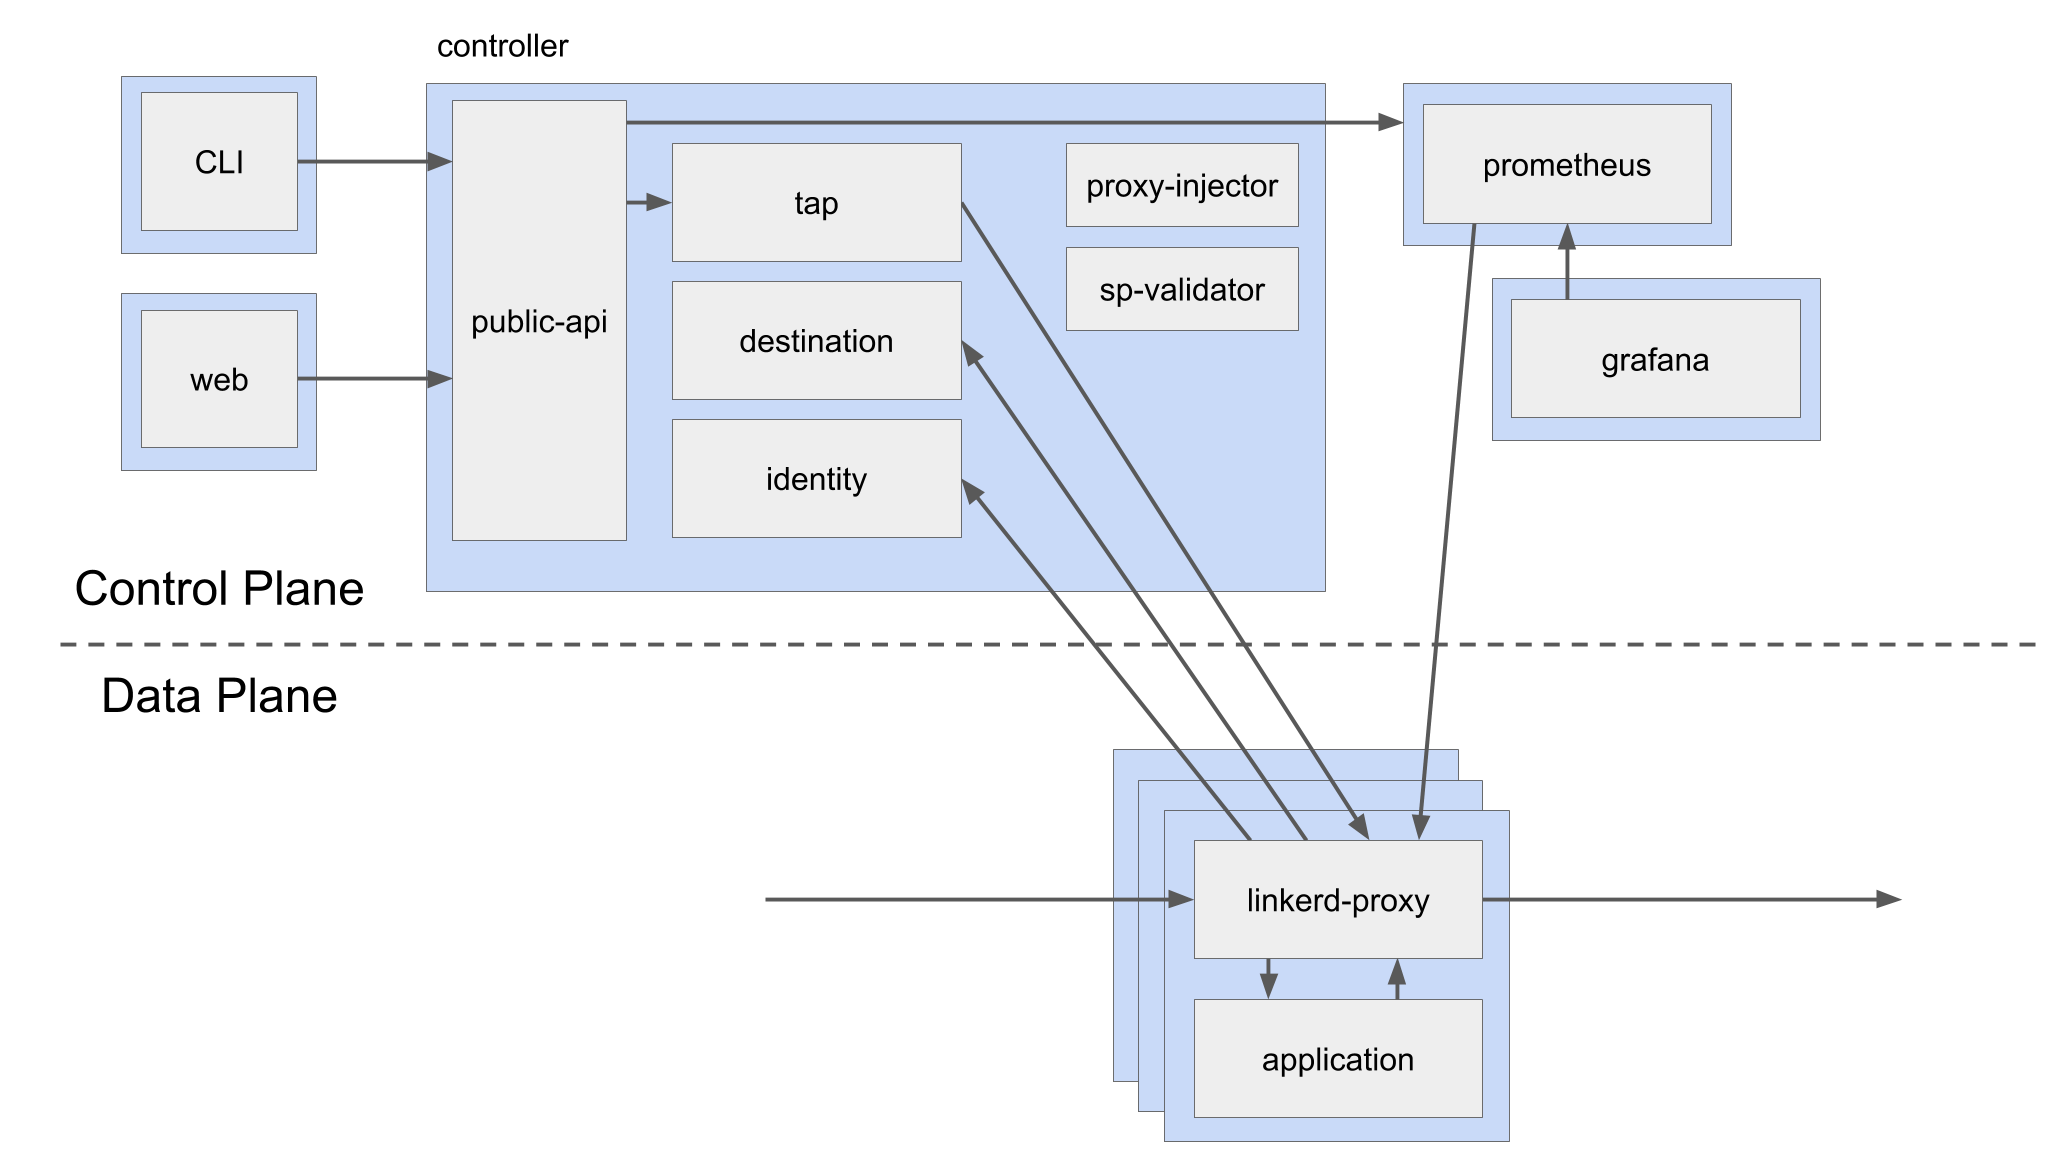
\includegraphics[width=\columnwidth]{img/linkerd_architecture.png}
    \caption{Architecture of Linkerd \cite{linkerd-docs-arch}}
    \label{fig:arch-linkerd}
\end{figure}

\subsection{Comparison}

As stated before, two very popular solutions for service meshes are Linkerd and Istio. Table \ref{tab:istio-linkerd} summarizes the key aspects of both tools, according to \cite{linkerd-github}, \cite{istio-github}, \cite{istio-linkerd-compare-1} and \cite{istio-linkerd-compare-2}:

\begin{table}
\centering

\begin{tabular*}{\columnwidth}{c|c|c}
                                 & Istio                                                                                                              & Linkerd     \\\hline
Initiators & \begin{tabular}[c]{@{}c@{}}Lyft, IBM,\\Google\end{tabular}                                                          	& \begin{tabular}[c]{@{}c@{}}Buoyant, Cloud Native\\Foundation\end{tabular}                                                           \\\hline
License                 & \multicolumn{2}{c}{Apache 2.0}                                                                                                          \\\hline
Runs on                          & \begin{tabular}[c]{@{}c@{}}Kubernetes,\\VMs\end{tabular}                                                           & Kubernetes  \\\hline
Sidecar proxy                    & \multicolumn{2}{c}{Yes}                                                                                                          \\\hline
Supports mTLS                    & \multicolumn{2}{c}{Yes}                                                                                                          \\\hline
Certificate management           & \multicolumn{2}{c}{Yes}                                                                                                          \\\hline
Authentication and authorization & \multicolumn{2}{c}{Yes}                                                                                                          \\\hline
Blue/Green deployment            & \multicolumn{2}{c}{Yes}                                                                                                          \\\hline
Circuit breaking                 & Yes                                                                                                                & No          \\\hline
Fault injection                  & \multicolumn{2}{c}{Yes}                                                                                                          \\\hline
Rate limiting                    & \multicolumn{2}{c}{Yes}                                                                                                          \\\hline
Monitoring                       & \multicolumn{2}{c}{Yes, with Prometheus}                                                                                         \\\hline
Complexity                       & High                                                                                                               & Low         \\\hline
Starts on GitHub \cite{linkerd-github} \cite{istio-github}              & 26.2k & 6.6k        \\\hline
Open issues on GitHub \cite{linkerd-github} \cite{istio-github}                 & 817                                                                                                                & 257         \\\hline
Documentation                    & ++                                                                                                                 & +          
\end{tabular*}
\vspace{0.25mm}
\caption{Comparison between Isto and Linkerd}
\label{tab:istio-linkerd}
\end{table}


%
%
% Mehr Erklärung zu Linkerd?
%
%

From an operators perspective, Istio and Linkerd look quite similar. After installing the service mesh, there are two main usage aspects: One the one hand, operators need to inject sidecar proxies in the pods of the microservice. On the other hand, they need to apply pluggable resources in YAML format, that could define policies like the usage of TLS.

By executing the command listed in \ref{lst:istio}, all deployments from namespaceA automatically get a sidecar proxy injected, while listing \ref{lst:linkerd} shows the injection command of a single deployment when using Linkerd.

\begin{lstlisting}[language=bash,caption={Injection of sidecards into deployments of a namespace in Istio},label={lst:istio}]
#!/bin/bash
kubectl label namespace default \
	istio-injection=enabled
\end{lstlisting}

\begin{lstlisting}[language=bash,caption={Injection of sidecards into a deployment in Linkerd}, label={lst:linkerd}]
cat deployment.yml | linkerd inject - \
	| kubectl apply -f -
\end{lstlisting}

%
% TODO: WRITE STUFF
% 

In our prototypical implementation, we will use Linkerd as a service mesh technology. As table \ref{tab:istio-linkerd} clarifies, Linkerd seems to be less complex and more lightweight compared to Istio. One missing key feature of Linkerd is circuit breaking, which is requested by users and currently under development \cite{linkerd-circuit-breaker}. Nevertheless, Istio seems to be more powerful and mature, has more users and functionalities. Along with this, the pool of tutorials and documentation is also larger.
We will choose Linkerd because of its lightweight nature. The setup of Linkerd's hello world example looks pretty straight forward and suitable and appropriate for a proof of concept.